\documentclass[a4paper,11pt]{article}

% default margins are too big
\usepackage[a4paper,left=3cm,right=3cm,top=3cm,bottom=3cm]{geometry}

% gap of colummns
\setlength{\columnsep}{.5cm}

% fonts
\usepackage[utf8]{inputenc}
%\usepackage[francais]{babel}

% to get hyphenation on accented words
\usepackage[T1]{fontenc}

% href
\PassOptionsToPackage{hyphens}{url}\usepackage{hyperref}
\hypersetup{
    colorlinks=true,
    linkcolor=blue,
    filecolor=blue,      
    urlcolor=blue,
    bookmarks=true
}

% dialogues
\usepackage{dialogue}

% quotes
\usepackage{csquotes}

% code highlighting
\usepackage{minted}
\usemintedstyle{pastie}

% asm
\usepackage{amsmath}
\usepackage{amssymb}
\usepackage{amsthm}

% inline code
\usepackage{listings}
\usepackage{xcolor}

% tables
\usepackage{booktabs}

% algorithm
\usepackage[]{algorithm2e}

% for right cases
\newenvironment{rcases}
  {\left.\begin{aligned}}
  {\end{aligned}\right\rbrace}
  
% images
\usepackage{graphicx}
\usepackage{float}
\usepackage{wrapfig}

% quotes with small margin
\usepackage[font=small,skip=5pt]{caption}

% diagrams
\usepackage{tikz}
\usetikzlibrary{matrix}
\usetikzlibrary{positioning}

% for centered verbatim
\usepackage{fancyvrb}

% tables
\usepackage{booktabs}

% no identation
\setlength{\parindent}{0pt}

% theorem
\newtheorem{definition}{Definition}
\newtheorem{property}{Property}
\newtheorem{theorem}{Theorem}

% header
\title{Disco: Modern Session Encryption}
%\title{Noise + Strobe = Disco}
\author{David Wong}
\date{\emph{NCC Group}, \small{August 2018}}

% notes
\usepackage[disable]{todonotes}
%\setlength{\marginparwidth}{2cm}

% [[ and ]]
\usepackage{stmaryrd}

% references
\usepackage{biblatex}
\addbibresource{references.bib}

% images path
\graphicspath {{images/}}

% 
\begin{document}
\maketitle
\renewcommand{\abstractname}{Abstract}
\begin{abstract}
At Real World Crypto 2017, Joan Daemen won the Levchin Prize and announced that he believed permutation-based crypto was the future of symmetric cryptography. At the same conference Mike Hamburg introduced Strobe, a symmetric protocol framework capable of protecting sessions as well as building symmetric cryptographic primitives for the single cost of Joan Daemen's permutation Keccak. The next year, at Real World Crypto 2018 Trevor Perrin came to talk about the Noise protocol framework, a modern TLS-like protocol with similar traits but with a focus on flexibility, offering many handshake patterns to choose from in order to authenticate peers of a connection in different ways. Disco is the natural merge of the two projects, creating a new protocol based solely on two unique primitives: Curve25519 and the Keccak permutation (or more correctly its wrapper Strobe). Experimental results show that a library based on Disco can be implemented on top of these two cryptographic primitives with only a thousand lines of code. This, while offering both a flexible way to encryption sessions and a complete cryptographic library for all of an application's needs.\\
\\
\textbf{Keywords:} Session Encryption, Embedded Devices, SHA-3, Keccak, Duplex construction, Permutation-Based Cryptography, Strobe, Noise, Protocol Framework, Disco, SSL, TLS\\

\end{abstract}
\vfill

\section{Introduction}\label{introduction}

The SHA-3 competition\cite{sha3} started more than 10 years ago and came to an end in 2012 with the nomination of the Keccak\cite{fips202} algorithm built from a sponge construction hosting a permutation at its core. Later, a more generic construction was invented called the duplex construction\cite{duplex}, which led to the invention of the Strobe protocol framework\cite{strobe}, a wrapper around the construction that can be used to construct symmetric protocols. On the other side of the field, the Noise protocol framework\cite{noise} is a project aiming at making the creation of secure protocols (like SSL/TLS) more flexible, easier to analyze and easier to implement. This paper attempts to merge the two frameworks Noise and Strobe into what we call Disco, a complete protocol framework aiming at simplifying secure protocols and minimizing the need to rely on several cryptographic primitives. The result of this experiment is a cryptographic library that holds in 1000 lines of code. The library can be used to setup (flexible) secure communications between endpoints and as a typical cryptographic library for operations like hashing, deriving keys, signing, encrypting, authenticating, etc.

Section 2 introduces the algorithm behind SHA-3 (a sponge and a permutation), while section 3 presents a similar construction (the duplex construction) and one of its real world applications (Strobe). Section 4 summarizes the efforts behind the Noise protocol framework. Finally, section 5 merges the effort from the previous two sections into one: Disco. Section 6 concludes with experimental results.

\section{SHA-3 and Keccak}

In 2007, the NIST organized the SHA-3 competition\cite{sha3}. Unlike the SHA-1 and SHA-2 algorithms that had previously been designed by the NSA, SHA-3 would be open to anyone willing to publicly share their design. 64 teams from all around the world entered the competition in hopes of becoming the new Secure Hashing Algorithm. Five years later, in 2012, Keccak (invented by a Belgian/Italian team including Guido Bertoni, Joan Daemen, Michaël Peeters and Gilles Van Assche) was designated as the winner\cite{fips202}. The other candidates who made it to the last round were BLAKE, Grøstl, JH, Skein.\\

While the NIST had many reason to choose Keccak, an interesting one was its departure in design from previously seen hash algorithms. Indeed, Keccak is built from a sponge, a construction that was invented during the course of the competition. 

\begin{figure}[H]
\centering
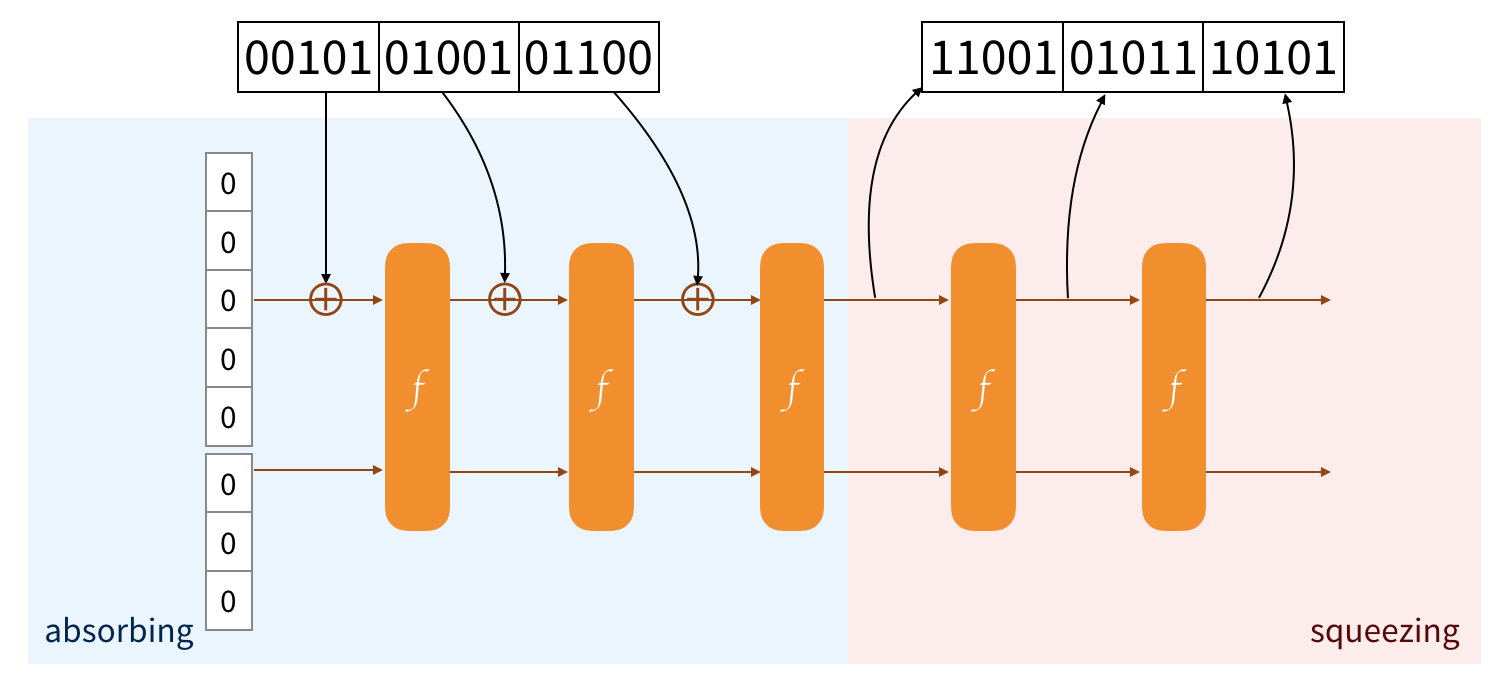
\includegraphics[width=0.8\textwidth]{rwcimg/sponge.png}
\caption{A simplified representation of the sponge construction.}
\label{fig:sponge}
\end{figure}

As can be seen in Figure \ref{fig:sponge}, a sponge is a very simple construction. A permutation $f$ takes an input state of size $b$ (8 bits in the above example) and randomizes it. It is used repeatedly to take on a larger initial input by way of XOR'ing. Recall that our construction is a sponge, so we naturally call this phase  "absorbing". To obtain an output, the permutation is used again until enough bits have been obtained, we naturally call this phase "squeezing". The security of the construction comes from the segregation applied to input and output states of the permutation: their first part (top, of 5 bits in our example) is called the \textbf{rate}, their second part (bottom, of 3 bits in our example) is called the \textbf{capacity}. As can be observed, the capacity is never touched and only the rate is mixed with the original input and read to produce the final output. More details (like padding, size of the capacity, etc.) are involved but for the sake of simplicity we omit them here.

A full security proof exists over the security of the sponge, provided that the permutation used in the construction has no structural distinguishers. Unfortunately, we have no known ways of proving this property and as with the study of block ciphers, cryptanalysts must be invoked and thrown at the algorithm for years in order to obtain an estimation of its security posture as well as to tweak its parameters. As the inventors of Keccak had experience with block ciphers --Joan Daemen being the co-inventor of AES (with Vincent Rijmen)-- the design of \textbf{Keccak-f} (Keccak's permutation) follows similar patterns.

\section{The duplex construction and Strobe}

One can wonder if there must only be one absorbing phase and one squeezing phase. And indeed, a construction introduced as the sister of the sponge, called the duplex, breaks this boundary:

\begin{figure}[H]
\centering
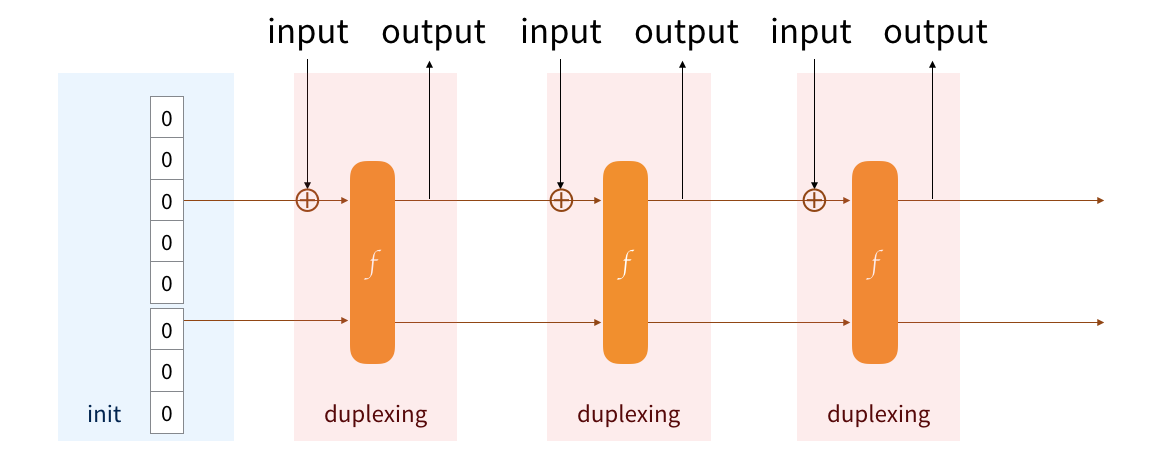
\includegraphics[width=0.8\textwidth]{rwcimg/duplex.png}
\caption{A simplified representation of the duplex construction.}
\end{figure}

While a set of formal proofs shows security equivalence to the sponge, the duplex construction is quite different in practice. It allows for the construction of more varied symmetric cryptographic primitives like re-seedable pseudorandom number generator, authenticated encryption schemes and the idea of sessions. The latter one encouraged the idea that a secure protocol could be formed around the construction, and thus the \textbf{Strobe protocol framework} was born. At its core is a set of public commands permitting access to the duplex functionalities by continuously mutating an internal state.

\begin{figure}[H]
\centering
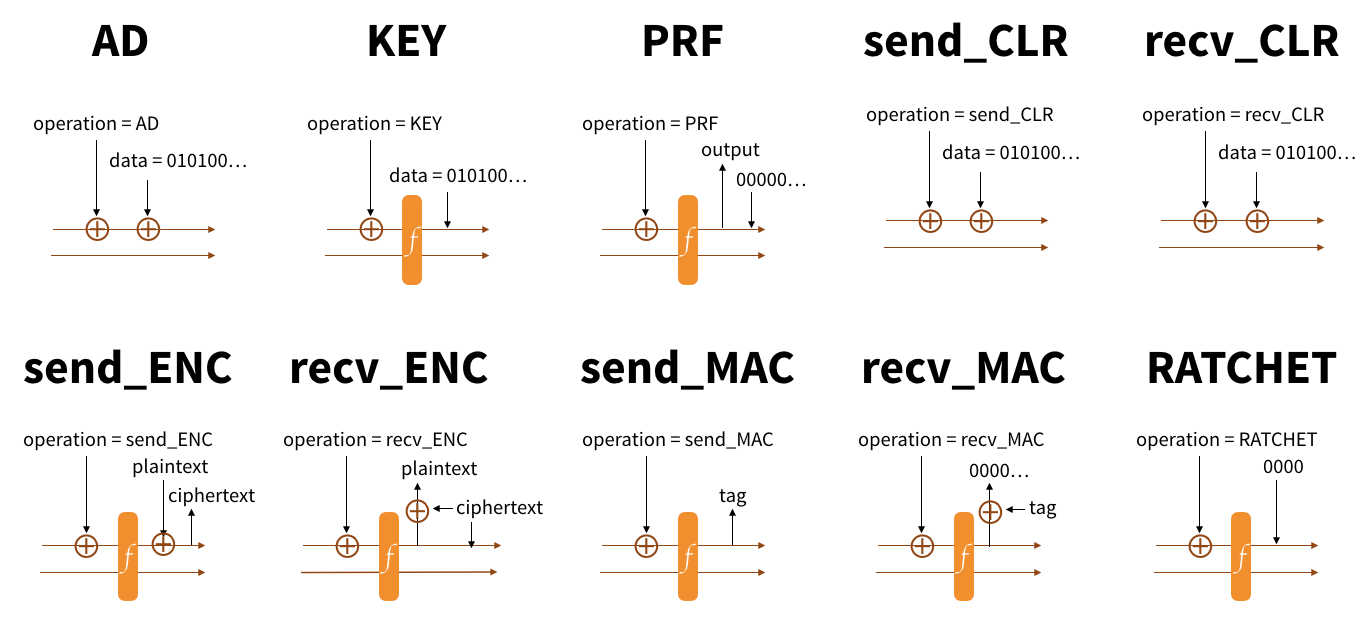
\includegraphics[width=\textwidth]{rwcimg/strobe.png}
\caption{All of the functions publicly exported by the API of Strobe.}
\label{fig:strobe}
\end{figure}

These commands can be combined (see figure \ref{fig:strobe}) to produce symmetric cryptographic primitives as well as to build more involved protocols. The Strobe protocol framework is first and foremost a specification around a standardized and common usage of the duplex construction. Once implemented, it typically takes around \textbf{a thousand lines of code}, and that includes the permutation Keccak-f as well. These two qualities make Strobe an excellent choice for embedded devices that have memory limitations as well as high-trust systems that do not want to rely on too many cryptographic primitives. In addition, implementations are easy to audit and to use as developers can consider Strobe as a black box.

\begin{figure}[H]
\centering
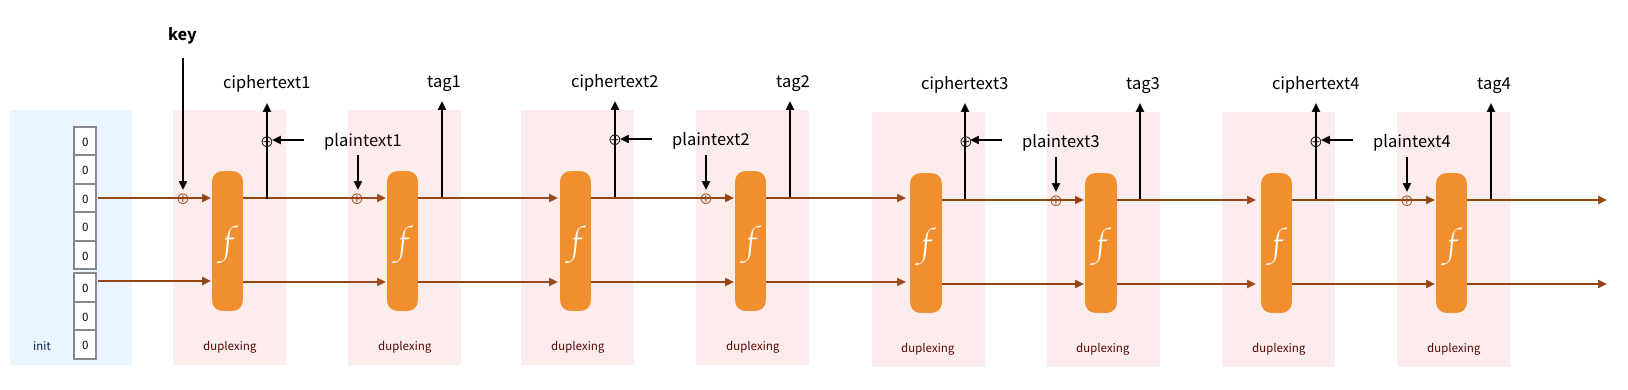
\includegraphics[width=\textwidth]{rwcimg/session.png}
\caption{A session built from the duplex construction. Each tag not only authenticate the previous encryption, but any operation that has happened prior to it.}
\end{figure}

The next section forgets about SHA-3, Keccak-f, the sponge and the duplex construction for a bit, but they will make a return (with Strobe) in section 5.

\section{The Noise Protocol Framework}

The Noise protocol framework is a specification\cite{noise} to build TLS-like protocols. One can implement only parts of it to form a secure communication protocol. While there are limited options for cryptographic primitives (X25519 or X448? Chacha20-Poly1305 or AES-GCM? SHA-256 or BLAKE2s?), the document specifies dozens of \textbf{handshake patterns} to chose from. These different patterns allow peers to authenticate each other in different ways, and will consequently provide different security properties at different point of the handshake. Once set on a handshake and a set of cryptographic primitives, the protocol is locked-in and can be implemented in a very linear way. All of this is described in the Noise specification as well as formally verified (with Tamarin\cite{tamarin}, ProVerif\cite{noiseexplorer} and CryptoVerif\cite{cryptoverif}) by different community efforts.\\

Handshake patterns are a series of directional messages containing tokens that must be digested one by one (on both sides of the connection) by a linear state machine. These patterns do not enforce the use of a public key infrastructure (PKI) and/or x.509 certificates and can be used to authenticate peers with plain keys, pre-shared secrets and even session fingerprints.\\

\begin{figure}[H]
\centering
\begin{BVerbatim}
NX:
  -> e
  <- e, ee, s, es
\end{BVerbatim}
\caption{The NX handshake pattern: both sides use ephemeral keys (\mintinline{python}{e}), but only the server authenticates itself by sending its long-term public key (\mintinline{python}{s}).}
\end{figure}

Implementers have to choose what pattern to use and implement the relevant subset of the specification. Once peers decide to eventually use the protocol to secure a communication, the handshake is started and each token is processed by the peers, dictating to them what needs to be done. For example, \mintinline{python}{e} means that the sender (resp. receiver) needs to generate an ephemeral keypair and send the public part (resp. receive a public key) whereas \mintinline{python}{es} means that a peer has to compute the Elliptic Curve Diffie-Hellman (ECDH) key exchange between the client's ephemeral key and the server's static key. Internally, a \textbf{running hash} $h$ continuously absorbs all messages that are being sent or received by the protocol, and is authenticated at the end of each turn, effectively providing transcript consistency to the session.

\begin{figure}[H]
\centering
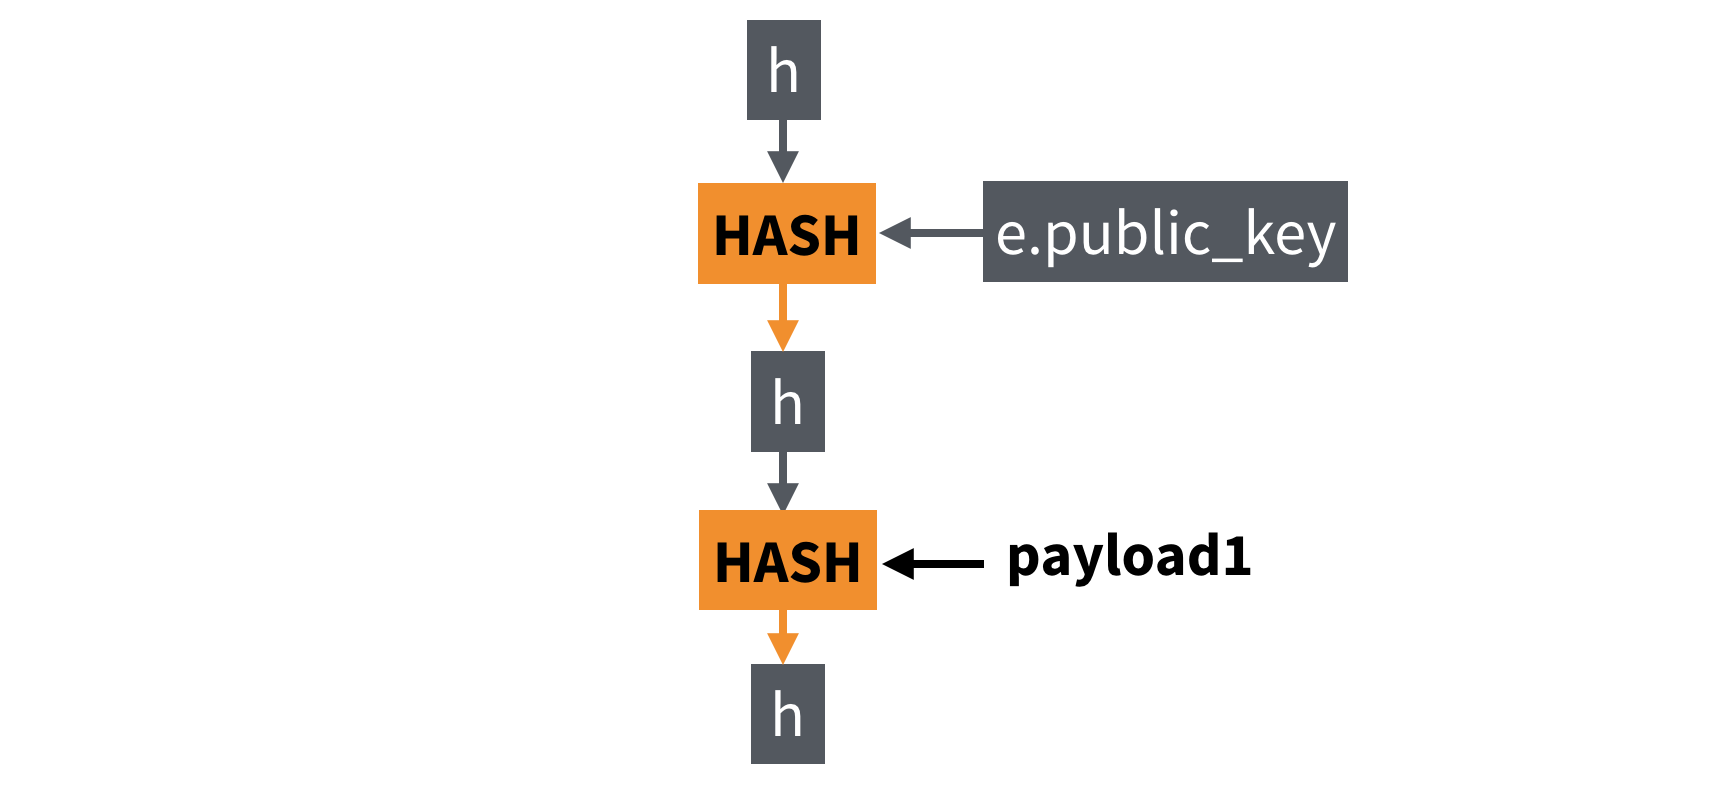
\includegraphics[width=0.5\textwidth]{rwcimg/h.png}
\caption{The running hash absorbs every message that transits through the network.}
\end{figure}

At the same time, a \textbf{chaining key} $ck$ is used continuously with outputs of the different key exchanges (that happen during the handshake) to derive new keys. These different keys are used to encrypt messages during and after the handshake.

\begin{figure}[H]
\centering
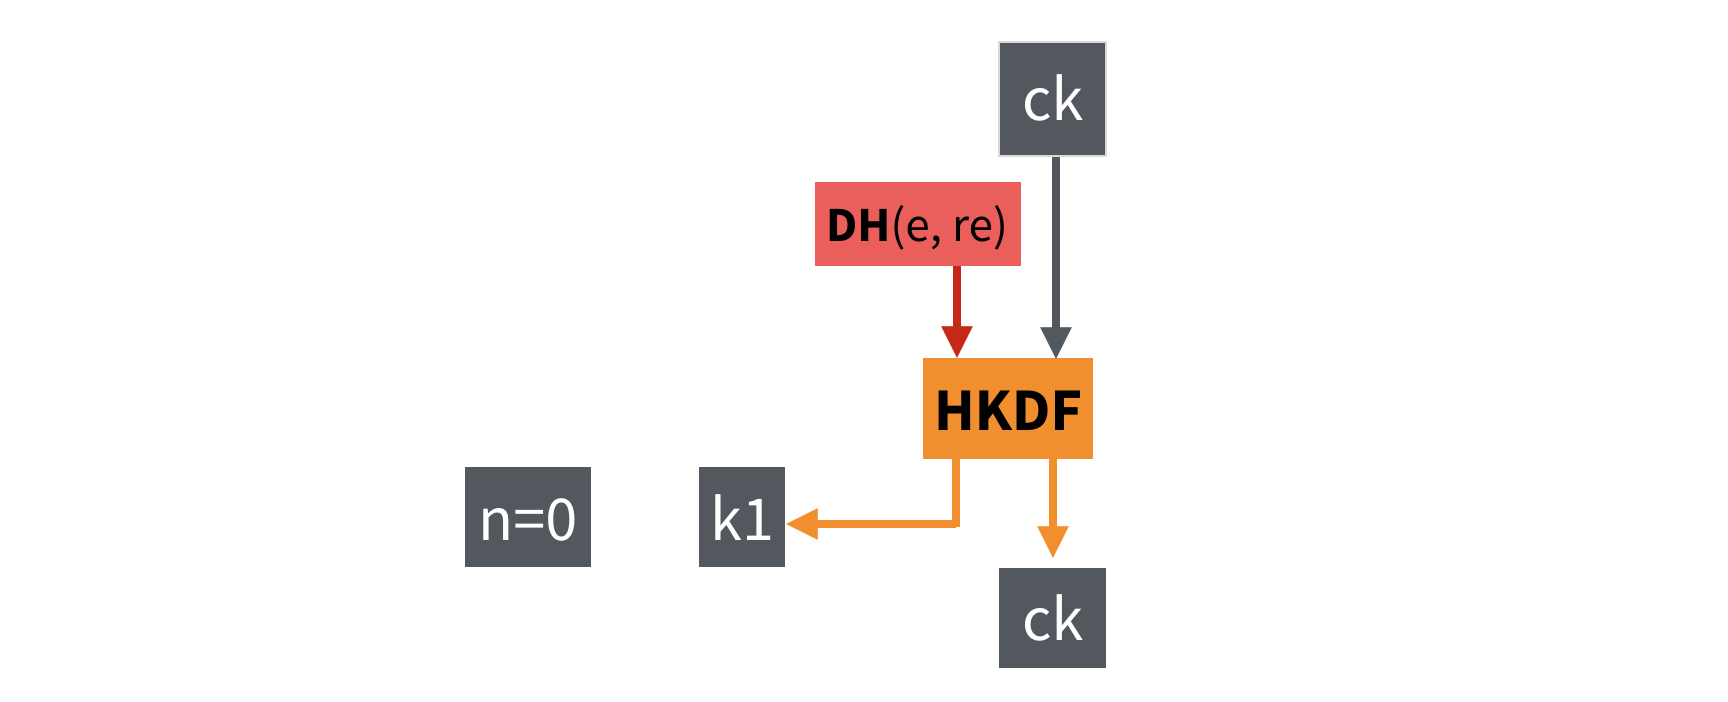
\includegraphics[width=0.5\textwidth]{rwcimg/ck.png}
\caption{The chaining key is given as input to HKDF along with the key exchange output, the result is used to derive an encryption key as well as the next chaining key.}
\end{figure}

The following dense diagram is a graphical simplified representation of the \emph{NX} handshake pattern, chosen to illustrate our work as it is closely resembling the typical TLS key exchange between a web browser and a web server.

\begin{figure}[H]
\centering
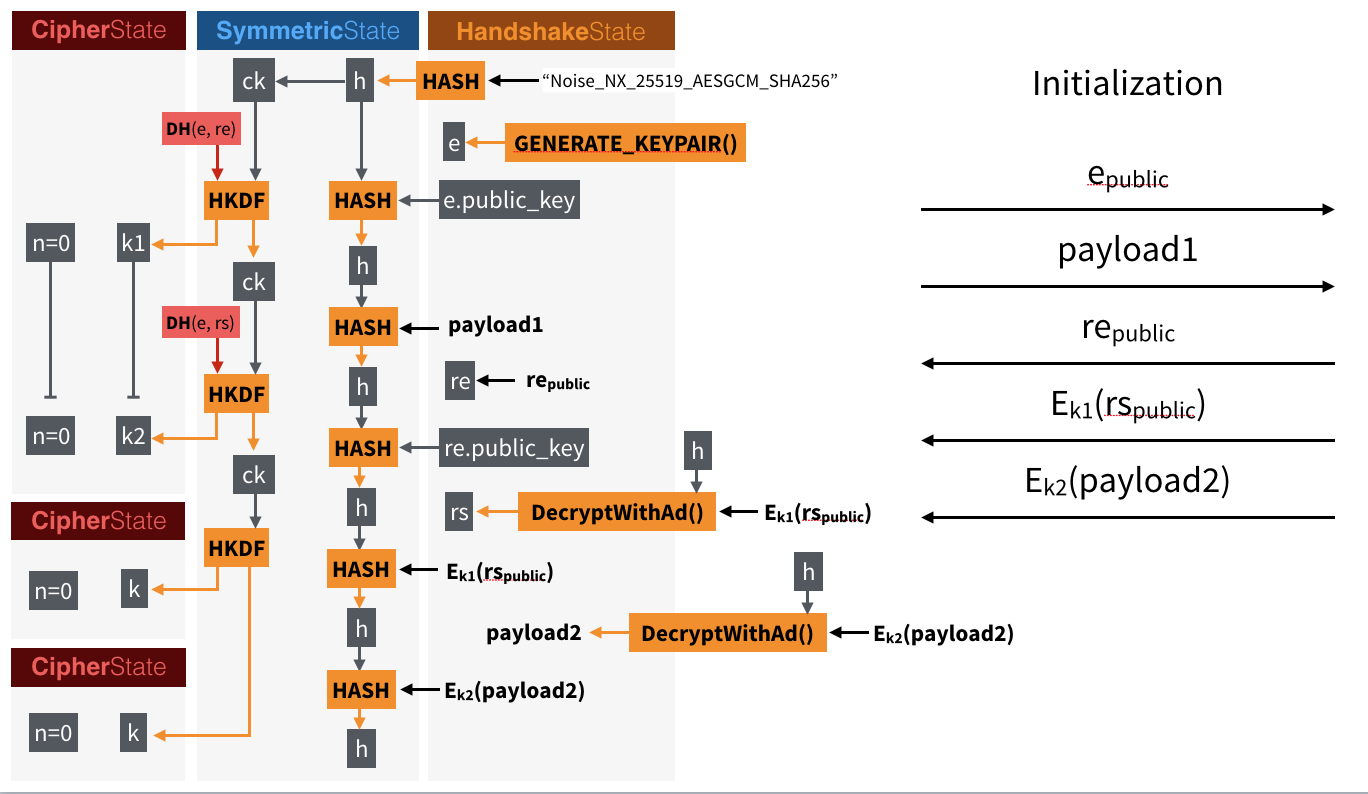
\includegraphics[width=\textwidth]{rwcimg/noise_nx.png}
\caption{A simplified representation of the \emph{NX} handshake pattern of the Noise protocol framework. As can be seen, three different states are maintained by a peer, one used to store asymmetric keys, one used to store the running hash and the chaining key, one used to store derived keys used for encryption.}
\label{fig:noise_nx}
\end{figure}

As can be seen, while the standard is quite simple compared to something like TLS, and while the state machine is truly linear, neither analyzing nor implementing the protocol appear to be straightforward tasks. The next section will attempt to use Strobe as a black box primitive in order to replace all of the symmetric primitives of Noise (HKDF, HMAC, SHA-2, BLAKE2, AES-GCM, Chacha20-Poly1305) with the Keccak-f permutation.

\section{Noise + Strobe = Disco}

In the description of the running hash $h$, we purposefully used the word "absorbing" to point out that a sponge or a duplex construction could be used. Furthermore, the duplex construction also supports the derivation of keys, re-seeding and authenticated encryption. This leads us to believe that Strobe could be used to replace all of the complex machinery we've seen in figure \ref{fig:noise_nx}.\\

Indeed, this is what we propose with our contribution, that we naturally call \textbf{Disco}.

\begin{figure}[H]
\centering
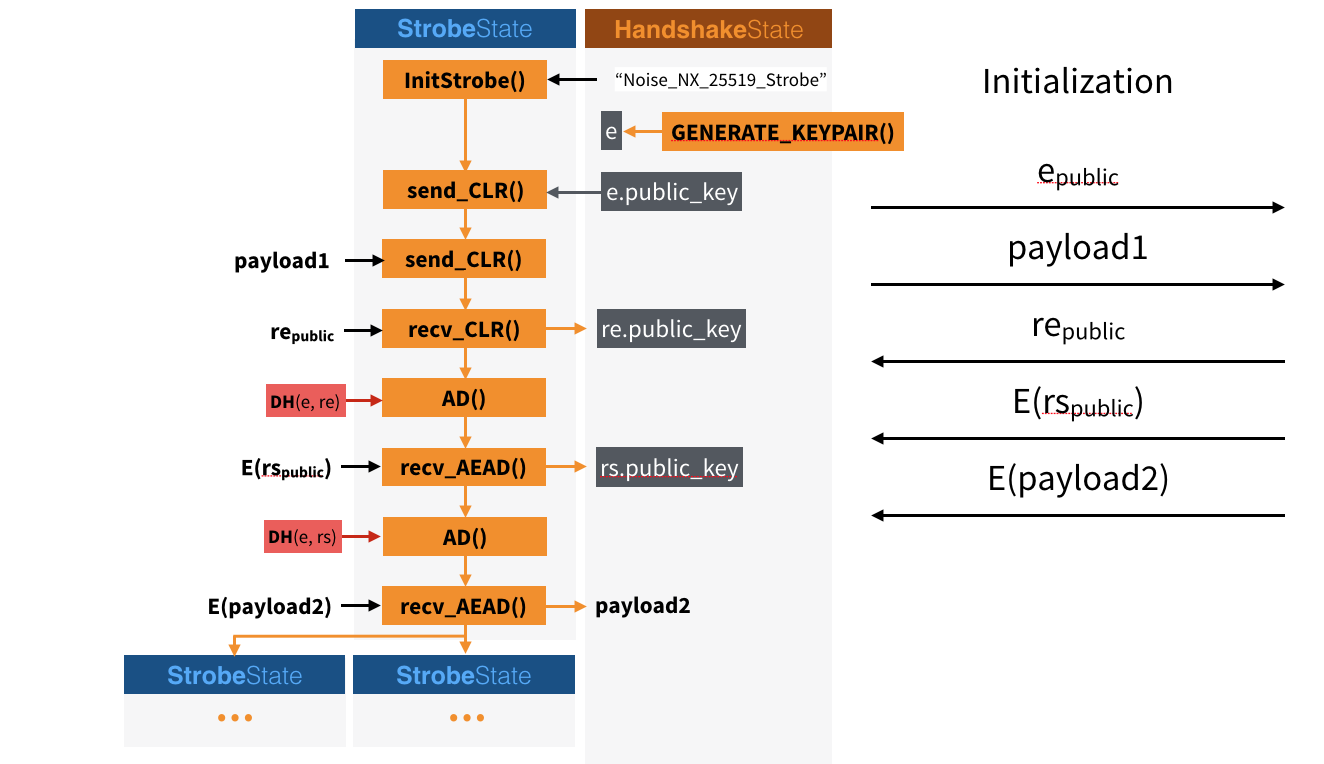
\includegraphics[width=\textwidth]{rwcimg/disco_NX.png}
\caption{The NX pattern within Disco. Both the CipherState and SymmetricState have been removed in favor of a unique and simple StrobeState.}
\end{figure}

The \mintinline{python}{send_CLR} (resp. \mintinline{python}{recv_CLR}) operation can be used to absorb messages being sent (resp. received) while the similar \mintinline{python}{AD} operation can be used to absorb key exchange outputs. \mintinline{python}{send_AEAD} and \mintinline{python}{recv_AEAD} are used to encrypt and decrypt messages. These functions do not exist in Strobe and are used as shorthands to represent a \mintinline{python}{send_ENC} (resp. \mintinline{python}{recv_ENC}) operation followed by a \mintinline{python}{send_MAC} (resp. \mintinline{python}{recv_MAC}) operation.\\

The duplex construction naturally absorbs every operation. No more key derivation is needed as encryption/decryption is influenced by everything that was absorbed previously. A stronger session consistency is obtained in the same way. Finally, we note that from an implementer's perspective, the protocol now seems drastically simpler. From a trust perspective, we now only rely on one single symmetric primitive: Keccak-f. 

The construction is so graceful that we can "zoom-in" and discern the internals of the duplex construction during the same handshake.

\begin{figure}[H]
\centering
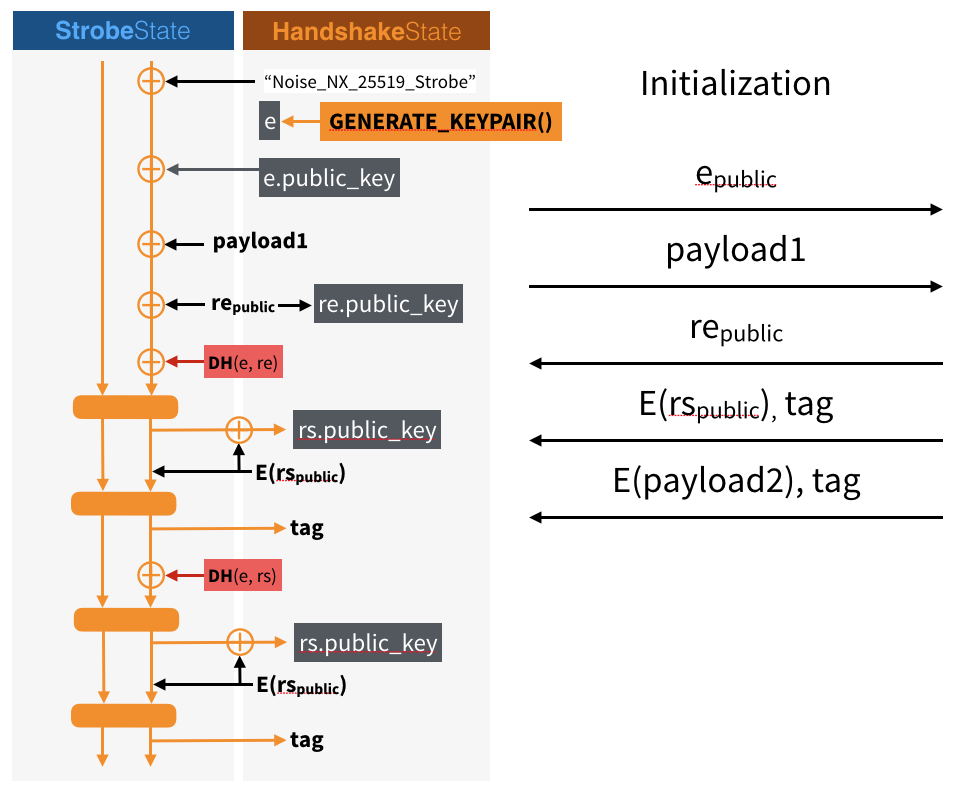
\includegraphics[width=0.7\textwidth]{rwcimg/duplex_view.png}
\caption{The Disco NX handshake pattern view from the inside. Absorption has been simplified: if the input is larger than the rate, the state needs to be permuted in between smaller absorptions.}
\end{figure}

Disco is currently being proposed as an extension to Noise\cite{disco}. It defines a new \mintinline{python}{SymmetricState} and a set of functions that acts on a stored Strobe state:\\

\mintinline{python}{InitializeSymmetric(protocol_name)} calls \mintinline{python}{InitializeStrobe(protocol_name)} on the Strobe state.\\

\mintinline{python}{MixKey(input_key_material)} calls \mintinline{python}{AD(input_key_material)} on the Strobe state.\\

\mintinline{python}{MixHash(data)} calls \mintinline{python}{AD(data)} on the Strobe state.\\

\mintinline{python}{MixKeyAndHash(input_key_material)} calls \mintinline{python}{AD(input_key_material)} on the Strobe state.\\

\mintinline{python}{GetHandshakeHash()} calls \mintinline{python}{PRF(32)}. This function should only be called at the end of a handshake, i.e. after the Split() function has been called. This function is used for channel binding\cite[Section 11.2]{noise}.\\

\mintinline{python}{EncryptAndHash(plaintext)} returns a ready to be sent payload to the caller by using the \mintinline{python}{send_ENC()} and \mintinline{python}{send_MAC()} functions on the Strobe state.\\

\mintinline{python}{DecryptAndHash(ciphertext)} returns the received payload by using the \mintinline{python}{recv_ENC()} and \mintinline{python}{recv_MAC()} functions on the Strobe state.\\

\mintinline{python}{Split()} clones the strobe state and differentiates each one of them via the recommendations given in \cite[Appendix C.1.]{strobe}. It then returns the pair of Strobe states for encrypting transport messages.\\

In practice, this \mintinline{python}{SymmetricState} transparently replaces Noise's \mintinline{python}{SymmetricState} and \mintinline{python}{CipherState}. More details are available on the specification of Disco itself\cite{disco}.

\section{Experimental Results}

To obtain a better understanding of our contribution, we have implemented Disco in Golang\cite{libdisco} and in C\cite{disco-c}. The process is pretty straightforward, first implement or re-use a Strobe library, then implement the Noise protocol framework (or modify an existing library) using the Disco specification.

The C implementation of Disco is around \textbf{1000 lines of code} which includes everything it needs: an X25519 implementation and Strobe (which contains an implementation of Keccak-f and a variant of Schnorr's signature algorithm with X25519). On the other hand, OpenSSL\footnote{\url{https://www.openssl.org/}} is around 700,000 lines of code and already lists 165 CVEs\footnote{\url{https://www.openssl.org/news/vulnerabilities.html}} on its page.

The Golang implementation was released as a more complete cryptographic library, offering a plug-and-play experience to connect two peers (with a choice of different handshake patterns) and a set of stand-alone cryptographic primitives for all of an application's need. Its implementation is 1000 lines of code. Add  Strobe (which contains an implementation of the Keccak-f permutation) and that's a total of 2000 lines of code. Add an implementation of X25519 and we end up with a total of 4000 lines of code. On the other hand, Golang's standard crypto/tls\footnote{\url{https://golang.org/pkg/crypto/tls/}} library is 5000 lines of code not including certificate parsing and the numerous cryptographic primitives it needs to operate.

More research needs to be done in order to benchmark the implementations and analyze their final codesize once deployed in different kind of devices and situations.

\section{Conclusion}

In this document We have introduced Disco, a simple protocol to encrypt sessions based on both Noise and Strobe. Disco can be implemented in only a thousand lines of code and its trust can be traced back directly to two solid cryptographic primitives: Curve25519 and Keccak-f. At the same time, thanks to the use of Strobe, an entire cryptographic library results from implementations of Disco. Future work includes proving the protocol formally, developing and testing new implementations of Disco, and standardizing the protocol as an RFC.

\section*{Acknowledgements}

Many thanks to Mike Hamburg and Trevor Perrin who are the two legs of this project.
\newpage
\printbibliography

\end{document}
